%!TEX root = ../crimson_throne_book_main.tex
% 2015-02-07
After they have recovered from the fierce battle with Mammy Graul and her undead ogre spouse, the companions search the rest of the homestead. With Puk still blinded and Balian still weakened by Mammy's necromantic magic, they proceed cautiously. The horrifying experience continues as they discover a dining room where the chairs are crowned with skulls and stretches with humanoid leather and a kitchen that has eyes and animal heads boiling in a stew. The stench of decaying flesh and excrement hangs thick throughout the building, accompanied by buzzing hosts of bloated flies. The young heroes confront one more hillbilly in the backroom. Although his frame clearly suggests that he is full-grown, the childish look in his eyes betrays his simple mindset. The hairless, malformed ogrekin smiles naively through his wide mouth of ragged teeth before he realizes that the men entering are intruders. He drops the humanoid baby skulls he was playing with and roars aggressively, flailing about wildly with his arms. Still, four adversaries and a dog prove too much of a challenge and he goes down easily. Quint draws back in horror as he examines the crude paintings in blood of grinning devils and dismembered animals on the walls, thinking of his horse that is still missing. Sjo ponders over the baby skulls: their grotesque shape makes him wonder whether these were ogrekin babies. Since all of Mammy Graul's children they have encountered so far were male, these small crania might be all that remains of her female offspring, toys for her sons. The upper floor proves less of a horror, housing one filthy bedroom and a junk-littered attic.\\

That leaves one more area to explore: the basement. The stairs lead down to a small hallway with three doors. The door on the right draws Balian's attention, as he hears the scraping sound of someone sharpening a weapon and the frightened whinnying of a horse. Puk attempts to push the door open, but finds it bolted from the other side, alarming the creatures in the room of the heroes' arrival. Quint quickly pulls the key-lock killer's magic bell from his pack and rings it, making the bolt pop free. The room reeks of rot and old blood. Piles of gore-spattered skin lie heaped on the floor. Quint's horse has been tied down to a large table, its legs are broken and it looks in bad shape, but still alive. A fierce-looking ogrekin towers over the table; hair grows lopsided from the right side of his head rather than atop his brow, but his left side reveals a more gruesome abomination: a second half-formed head grows from the back of his neck. It lacks the intelligent glare of the main head, though, and limits itself to grunting and drooling. The ogrekin orders two ratlike dogs to attack and roars out a threat in a language none of the heroes understand, although Quint recognizes it as {\itshape Giant} , the tongue used by ogres. In the other corner of the room, behind a second table, is Mammy Graul, who's shrieking encouragements at her son in Giant as well. Whatever she is yelling, it does not sound cordial, although Quint can make out that she calls the two-headed savage 'Hucker'. The\hyperref[fig:Grand-finale-in-the-Graul-homestead-basement-512310881]{ heroes rush across the room and engage the creatures } . Sjo focuses on the corpulent necromancer, noticing that most of the burns he inflicted earlier have been healed. His mace skitters off her layers of fat, but at least his presence menaces her enough to make her fizzle the spell she tries to cast. Puk stumbles forward blindly until he faces Hucker and one of the dogs. The luck of halflings protects him once more from the brute's deadly swing: the large metal hook tears into the ground instead of the unsighted rogue. At Quint's urging the halfling takes on a more defensive stance, since his puny attacks will not give the enemies more than a few scratches anyway. Meanwhile Balian and Spyder take out the second dog, but the ranger's decreased strength proves to be quite a handicap. Quint tries to support his friends by snapping around his whip and tripping Mammy and her son. The obese necromancer finds herself cornered by Sjo and resorts to her  {\itshape wand of magic missiles} , fearing to lose more spells in melee. Even though she can fire only two  {\itshape force} bolts at the Shoanti at a time, her continued efforts wear him down and finally force him to step back to heal himself. \\

\begin{figure}[h]
	\centering
	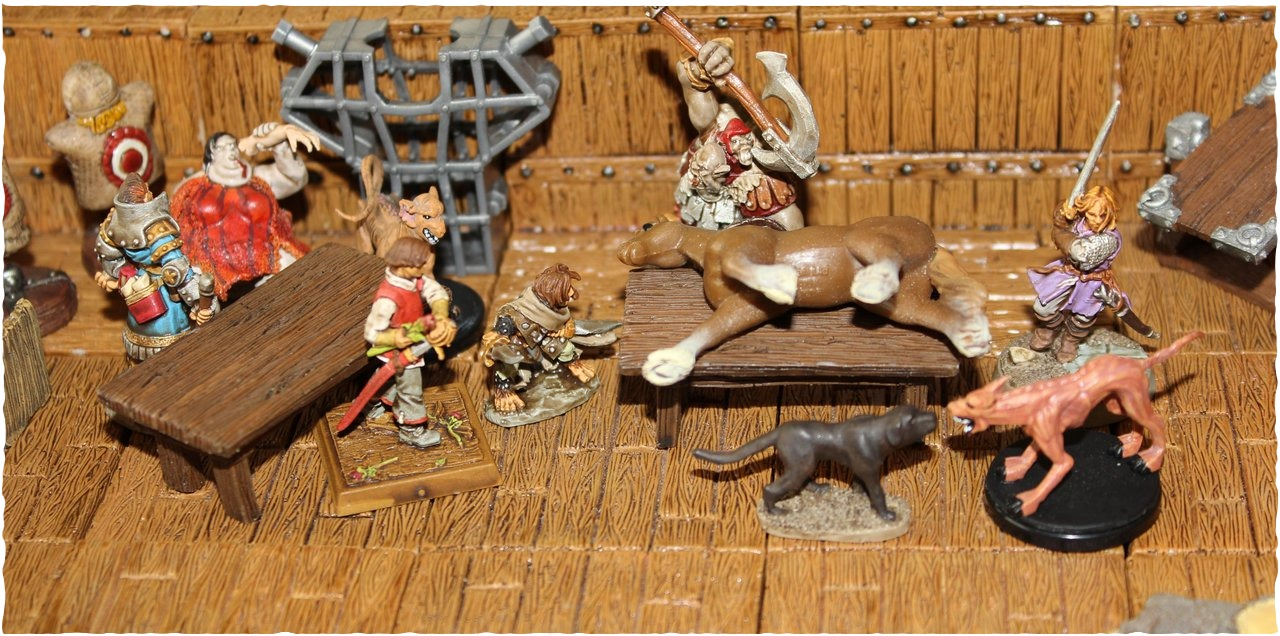
\includegraphics[width=0.4\textwidth]{images/Grand-finale-in-the-Graul-homestead-basement-512310881_mod.jpg}
	\caption{Grand finale in the Graul homestead basement}
	\label{fig:Grand-finale-in-the-Graul-homestead-basement-512310881}
\end{figure}

In the meantime the other heroes focus their attacks on the big ogrekin. Quint and Balian inflict several deep cuts, but the brute retaliates, dealing a mighty blow to Quint and hitting down Spyder. Balian presses the attack and finally finishes off Hucker with a critical strike. Sjo no longer has the magic to {\itshape outheal} Mammy and hits the floor as well. Once he ratdog has been taken care of, Mammy is the only adversary left. Hatred burns in her eyes as she keeps on firing  {\itshape magic missiles} at Puk now, who is next to lose consciousness. Balian now hits his greatsword into the fat monster's flesh, but it's Quint  {\itshape frosty} shortsword that delivers the final blow and ends this horrific conflict. The bard has just enough magic left to get Sjo and Puk back to their feet. Every potion, wand or spell that can provide healing has been depleted. Apart from Balian, who sustained no wounds in this last fight, all other heroes are barely alive. Getting some rest is a necessity, but first the companions make sure there are no more enemies about. Fortunately there aren't. As they search the rest of the basement, they find two more junk rooms and one large filthy prison that also serves as the building's cesspit. Manacled to the far wall is a strange man with goat-like legs and horns, a satyr. He is not conscious, although he is still breathing. His right arm has been chopped off, leaving only a bloody stump. This must have been the 'treat' Mammy Graul was chewing on when the heroes first surprised her. The companions free the faun and take him outside, where Sjo and Balian bind his wounds. The exhausted young adventurers spend the night in the barn at the side of their horses.\\

\section{3 Erastus 4708}

The companions take the rest of the day to recuperate and heal their wounds. Fortunately, Mammy Graul was smart enough to keep around at least one bottled cure to her own blinding magic in the form of a {\itshape potion of remove blindness} , which repairs Puk's sight, while Sjo's magic gives Balian his strength back. Quint's horse is healed of its broken legs and the heroes carefully bring back the satyr to consciousness. He is traumatized by this horrid experience, but Quint's kind words and music restore enough sanity so he can communicate. His name is Dernal, a satyr who lives here in the wilds. When he realizes that the threat has ended, he asks his rescuers if they have found his emerald necklace. This prompts a closer search of the lodge which reveals a secret cache in Hucker's basement room. A treasure chest holds some money and jewelry, as well as a pair of magical  {\itshape bracers of lesser archery} . 